\section{Implementation}\label{sec:implementaion}
%To demonstrate the use of Crypt$\epsilon$ primitives let us look at the following example.
\label{implementation}
In this section we describe the implementation of Crypt$\epsilon$. First we discuss our novel proposed technique for extending the $labMult$ operation of \textsf{labHE} to support $n > 0$ multiplicands. Then we describe the implementations for each primitive. Last, we use the example programs from the previous section to illustrate the performance of \system.

\subsection{\textbf{General n-way multiplication for \textsf{labHE}- $genLabMult()$}}\label{genlab}
\begin{algorithm}
\caption{$genLabMult$ - generate label for $labMult$}
\begin{algorithmic}[1]
\STATEx
\textbf{Input}: $\mathbf{c_1}=labEnc_{pk}(m_1),\mathbf{c_2}=labEnc_{pk}(m_2)$
\STATEx \textbf{Output}: $\mathbf{d}=labEnc_{pk}(m_1\cdot m_2)$
\STATEx \textbf{\textsf{AS}:} \STATE Computes $\textbf{d}'=labMult(\mathbf{c_1,c_2}) \oplus Enc_{pk}(r)$ where $r$ is a random mask \STATE Sends $\mathbf{d'},\mathbf{c_1},\mathbf{c_2}$ to \textsf{CSP}
\STATEx \textbf{\textsf{CSP}:}
\STATE Decrypts $\mathbf{d'}$, to get $Dec_{sk}(\mathbf{d}')=m_1\cdot m_2 -b_2\cdot b_1 + r$
\STATE Computes $b_1 \cdot b_2$ from the labels of $\mathbf{c_1}$ and $\mathbf{c_2}$.
\STATE Removes $b_1\cdot b_2$ from $d'$ to compute $d''=m_1\cdot m_2+r$
\STATE Picks a seed $\sigma'$ and label $\tau'$
\STATE Computes $\bar{a}=m_1\cdot m_2 -b' +r$, $b'=\mathcal{F}(\sigma',\tau')$ and $\mathbf{b'}'=Enc_{pk}(b')$
\STATE Send $\bar{d}=(\bar{a},\mathbf{b'})$ to \textsf{AS}\STATEx \textbf{\textsf{AS}:}
\STATE Computes true cipher $\mathbf{d}=(a',\mathbf{b}')$ where $a'=\bar{a}-r=m_1\cdot m_2 - b'$
 \end{algorithmic}
\end{algorithm}
Consider the case where we want to multiply the respective ciphers of  $n$ messages $\{m_1,...m_n\} \in \mathcal{M}^n$. Note that the reason why we can't simply use $labMult$ for a generic $n-$ way multiplication is because, the "multiplication" cipher $\mathbf{d}=labMult(\mathbf{c_1},\mathbf{c_2})$ does not have  a corresponding label. Thus for generalizing the $labMult$ operation for $n$ multiplicands what we have to do is to generate a label and a seed for every intermediary product of two multiplicands. This can be done as shown by Algorithm 1. Note that the mask $r$ protects the value of $m_1\cdot m_2$ from the \textsf{CSP} in step 5. Similarly since $b'$ is not known to the \textsf{AS}, $m_1\cdot m_2$ remains hidden from the \textsf{AS} in step 9. Now with the true \textsf{labHE} cipher $\mathbf{c}=(a',c')$ for the product the \textsf{AS} can compute further multiplications on it.
For a generic $n-way$ multiplication the order of multiplication can be, in fact, parallelized as  shown in Figure ~\ref{genlab-fig} to require a total of $\lceil \log n\rceil$ rounds of communication with the \textsf{CSP}.
\begin{figure}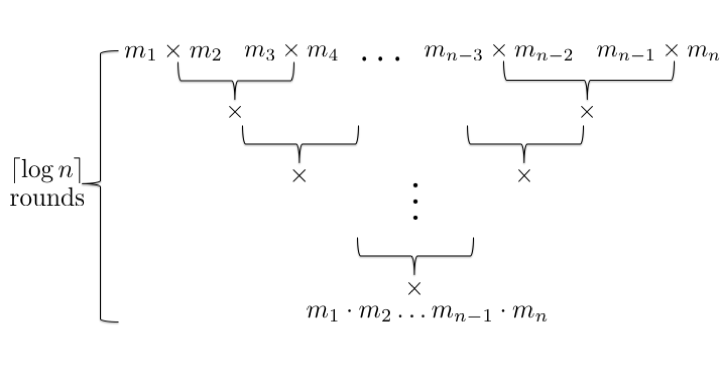
\includegraphics[height=4cm,width=8cm]{kk.png} \caption{ $genLabMult()$ - Batching of multiplicands for \textsf{labHE}} \label{genlab-fig}\end{figure}\\


\subsection{Primitive Implementation}
%Now let us explain the implementation details of the aforementioned Crypt$\epsilon$ primitives.  
In this section we explain the implementation details of two of the aforementioned \system primitives, the rest are covered in appendix section B.\\ \textbf{\textsf{GroupByCount }}$\groupbystar_A(\mathbf{\tilde{T}})$- The \textsf{GroupByCount} primitive is implemented  goes as follows   \begin{enumerate}[label=\alph*)]\item $\mathbf{V}=\groupbystar_{A}(\boldsymbol{\tilde{\mathcal{D}}})$ \\
 Note that since each entry of $\mathbf{V}$ is a count of records, its value ranges from $\{0,...,m\}$. \item \textsf{AS} creates a mask vector $M$ drawn uniformly at random from $[m]^{s_A}$, i.e.,  \begin{gather*} M[i] \in_R [m], i \in [|V|]\end{gather*} \item \textsf{AS} masks the encrypted true count vector $\mathbf{V}$ for attribute $A$ as follows \begin{gather*}\boldsymbol{\mathcal{V}}[i]= \mathbf{V}[i] \oplus labEnc_{pk}(M[i])\end{gather*} and sends $\boldsymbol{\mathcal{V}}$ to \textsf{CSP}.\item \textsf{CSP} decrypts $\boldsymbol{\mathcal{V}}$, converts each entry to its corresponding one-hot-coding and encrypts it. \begin{gather*}\mathcal{V}[i]=labDec_{sk}(\boldsymbol{\mathcal{V}})\\\tilde{\mathcal{V}[i]}=\mathcal{E}(\mathcal{V}[i])[\text{Generates one-hot-coding  }]\\\boldsymbol{\tilde{\mathcal{V}}}[i]=labEnc_{pk}(\tilde{\mathcal{V}[i]})\end{gather*}\item Notice that each entry of $\boldsymbol{\tilde{\mathcal{V}}}$ is a $m$ -lengthed one-hot-coding vector. \textsf{AS} now simply rotates every entry by its corresponding mask value to obtain the desired  encrypted one-hot-coding $\boldsymbol{\tilde{V}}[i]$. \begin{gather*}\boldsymbol{\tilde{V}}[i]=RightRotate(\boldsymbol{\tilde{\mathcal{V}}},M[i])\end{gather*}  \end{enumerate} Note that the \textsf{GroupByCount} primitive could have an alternative implementation using a Yao's garbled circuit that takes an input the encrypted vector and outputs the corresponding one-hot-coding representation. However this would require the circuit to decrypt and re-encrypt $O(m)$ data inside it which would be computationally heavy for larger values of $m$. 
 \\ \textbf{\textsf{Laplace }}$\lap_{\epsilon,\Delta}(\mathbf{V})$ - Recall that both \textsf{AS} and \textsf{CSP} have to add Laplace noise to the output in Crypt$\epsilon$. Hence the \textsf{Laplace} primitive has two components. The first component is executed by the \textsf{AS} wherein,
\begin{enumerate} \item \textsf{AS} generates a noisy vector $\eta$ such that $\eta \in [Lap(\frac{1}{\epsilon})]^{|V|}$ \item encrypts $\eta$ and adds it to the input vector as \begin{gather*}\boldsymbol{\eta}=labEnc_{pk}(\eta)\\\mathbf{\hat{V}}[i]=\mathbf{V}[i]\oplus \boldsymbol{\eta}[i], i \in [|V|]\end{gather*} \end{enumerate} This encrypted noisy vector $\mathbf{\hat{V}}$ is the input for the second phase of the \textsf{Laplace} primitive which is executed by the \textsf{CSP} as follows \begin{enumerate}\item Decrypts $\mathbf{\hat{V}}$ \begin{gather*}\hat{V}=labDec_{sk}(\mathbf{\hat{V}})\end{gather*}  \item Generates a noisy vector $\eta'$ such that $\eta' \in [Lap(\frac{1}{\epsilon})]^{|\hat{V}|}$ \item Finally adds the noise $\eta'$ to $\hat{V}$ \begin{gather*}\hat{\mathcal{V}}[i]=\hat{V}[i]+\eta'[i], i \in [|\hat{V}|]\end{gather*} \item Returns $\hat{\mathcal{V}}$ to \textsf{AS} \end{enumerate} The implementation when the input is an encrypted scalar $\encC$ instead, is similar to the one presented above.

\subsection{Classification of \system Programs}
Crypt$\epsilon$ programs can be classified into three classes based on the number and type of interaction required between the \textsf{AS} and the \textsf{CSP}.  \\
\stitle{\textbf{Class I - Single Decrypt Interaction Programs:}}\\
Recall that the output of all the transformation primitives are encrypted.  Since  the \textsf{CSP} has exclusive access to the secret key, it is the only entity in the Crypt$\epsilon$ setting capable of decryption. Thus for releasing any result (albeit noisy) in the clear, we need to interact at least once with the \textsf{CSP} so that it can decrypt the encrypted noisy answer. Crypt$\epsilon$ supports this type of interactions via the two measurement primitives. Some Crypt$\epsilon$ programs require only this one round of interaction at the very end to release the noisy output. All other transformations can be performed by the \textsf{AS} via homomorphic operations on the encrypted data records. Typically these programs are counting queries on a single attribute or noisy max on a single attribute. Examples of this type of programs are P1 and P2 from Table \ref{tab:programexamples}.\\
\stitle{\textbf{Class II : \textsf{LabHE} Multiplication Interaction Programs-}}\\
Recall that labeled homomorphic encryption allows multiplication of two ciphers. Generalization to a $n$-multiplicand, $n > 2$ case can be done according to the protocol described in section \ref{genlab}. However it requires intermediate interactions with the \textsf{CSP}. Thus all Crypt$\epsilon$ programs that require multiplication of more than two ciphers need interaction with the \textsf{CSP}. 
All programs with more than three attributes in its boolean predicate would thus fall under this class. P3, P4 and P5 from table 3 fall in this class of \system programs.\\
\stitle{\textbf{Class III : Other Interaction Programs-}}\\
 The \textsf{GroupBy} primitive requires an intermediate interaction with the \textsf{CSP} (for generating the encrypted one-hot-coding). The \textsf{CountDistinct} primitive also uses a Yao's garbled circuit (see section C) and hence requires  interaction with the \textsf{CDP}. This in addition to the interaction required for decrypting the noisy answer (as explained above). Thus any program with the \textsf{GroupBy} or \textsf{CountDistinct} primitive requires two rounds of interaction in the least. P6 and P7 from Table \ref{tab:programexamples} are examples of this class of \system programs. 
